\documentclass{article}
\usepackage[utf8]{inputenc}
\usepackage{multicol}
\usepackage{graphicx}
\providecommand{\abs}[1]{\lvert#1\rvert}
\providecommand{\norm}[1]{\lVert#1\rVert}

\title{Tarea 3 Métodos Computacionales}
\author{Santiago Barreto Naranjo\thanks{s.barreto10@uniandes.edu.co}\\\textit{\small{Departamento de Física}}\\\textit{\small{Universidad de los Andes - Bogotá, Colombia }}}
\date{20/julio/2017}

\begin{document}

\maketitle


En el presente documento se muestran los resultados de la tercera tarea de métodos computacionales, los resultados corresponden a dos ejercicios que se realizaron en diferentes códigos tanto de python como de C. \\

\section{Primer punto}

En el primer caso encontramos la resolución de la ecuación de onda en dos dimensiones para una onda en una caja cuadrada de 30x30.\\



Esta imagen corresponde a la onda en un tiempo de 30 segs, que es el primer tiempo a examinar \\

\begin{center}
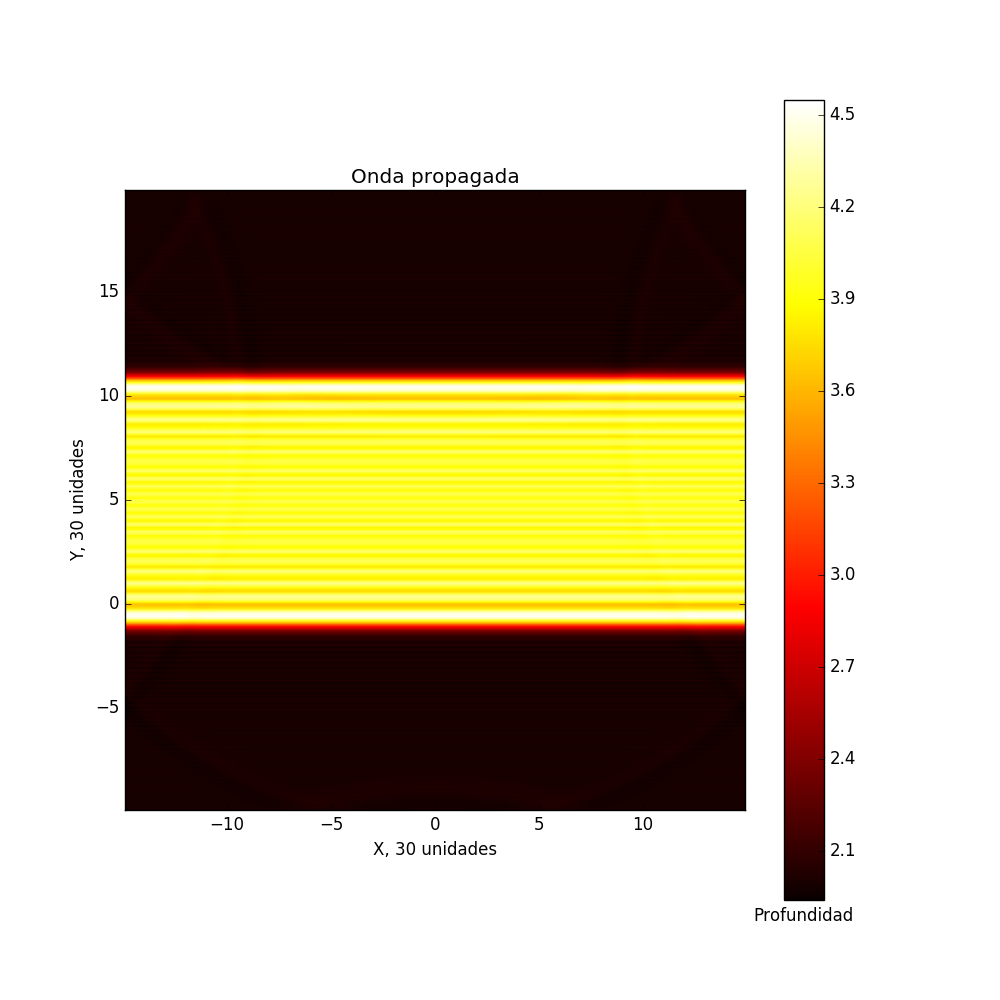
\includegraphics[scale=0.60]{t_1.png}
\end{center}

Esta imagen corresponde a la onda en un tiempo de 60 segundos, el tiempo final en el que se examina la onda:\\

\begin{center}
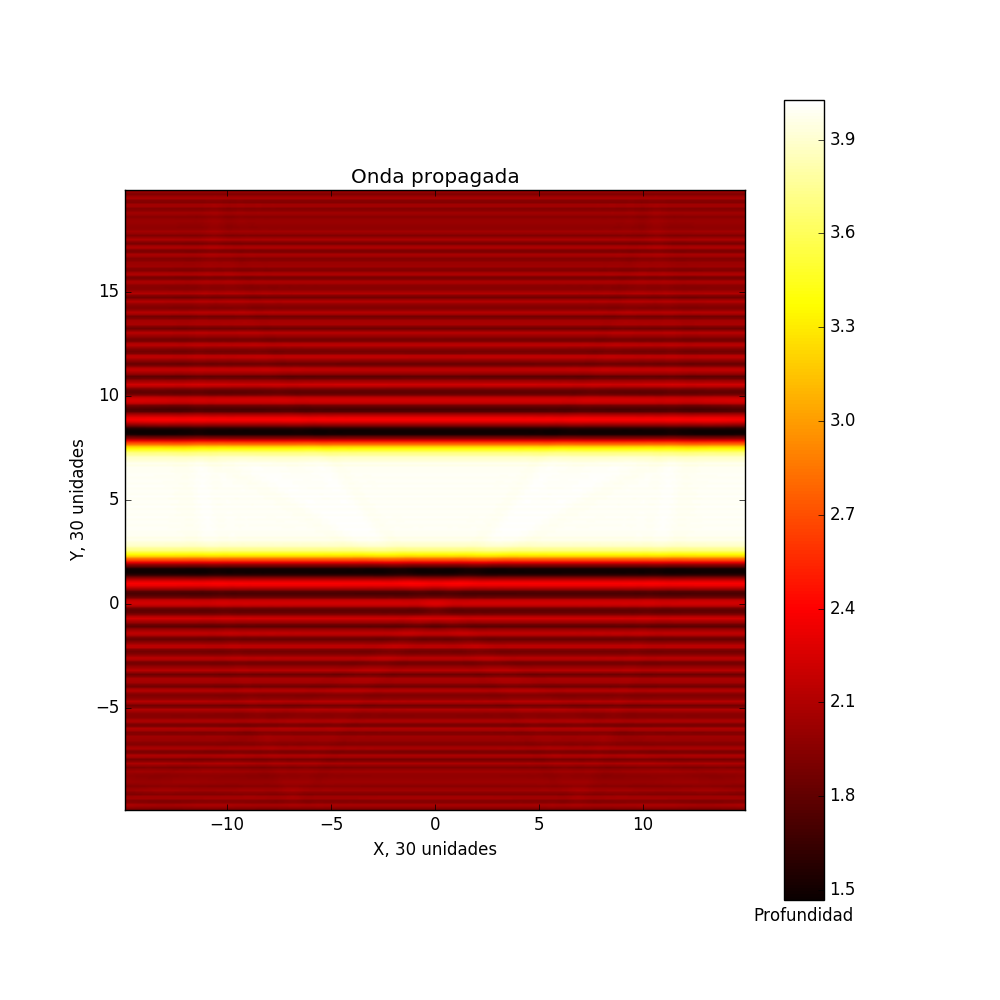
\includegraphics[scale=0.60]{t_f.png}
\end{center}

\section{Segundo punto punto}

\end{document}
